\begin{figure}[h]
    \centering
    % Top figure
    \begin{subfigure}[b]{\textwidth}
        \centering
        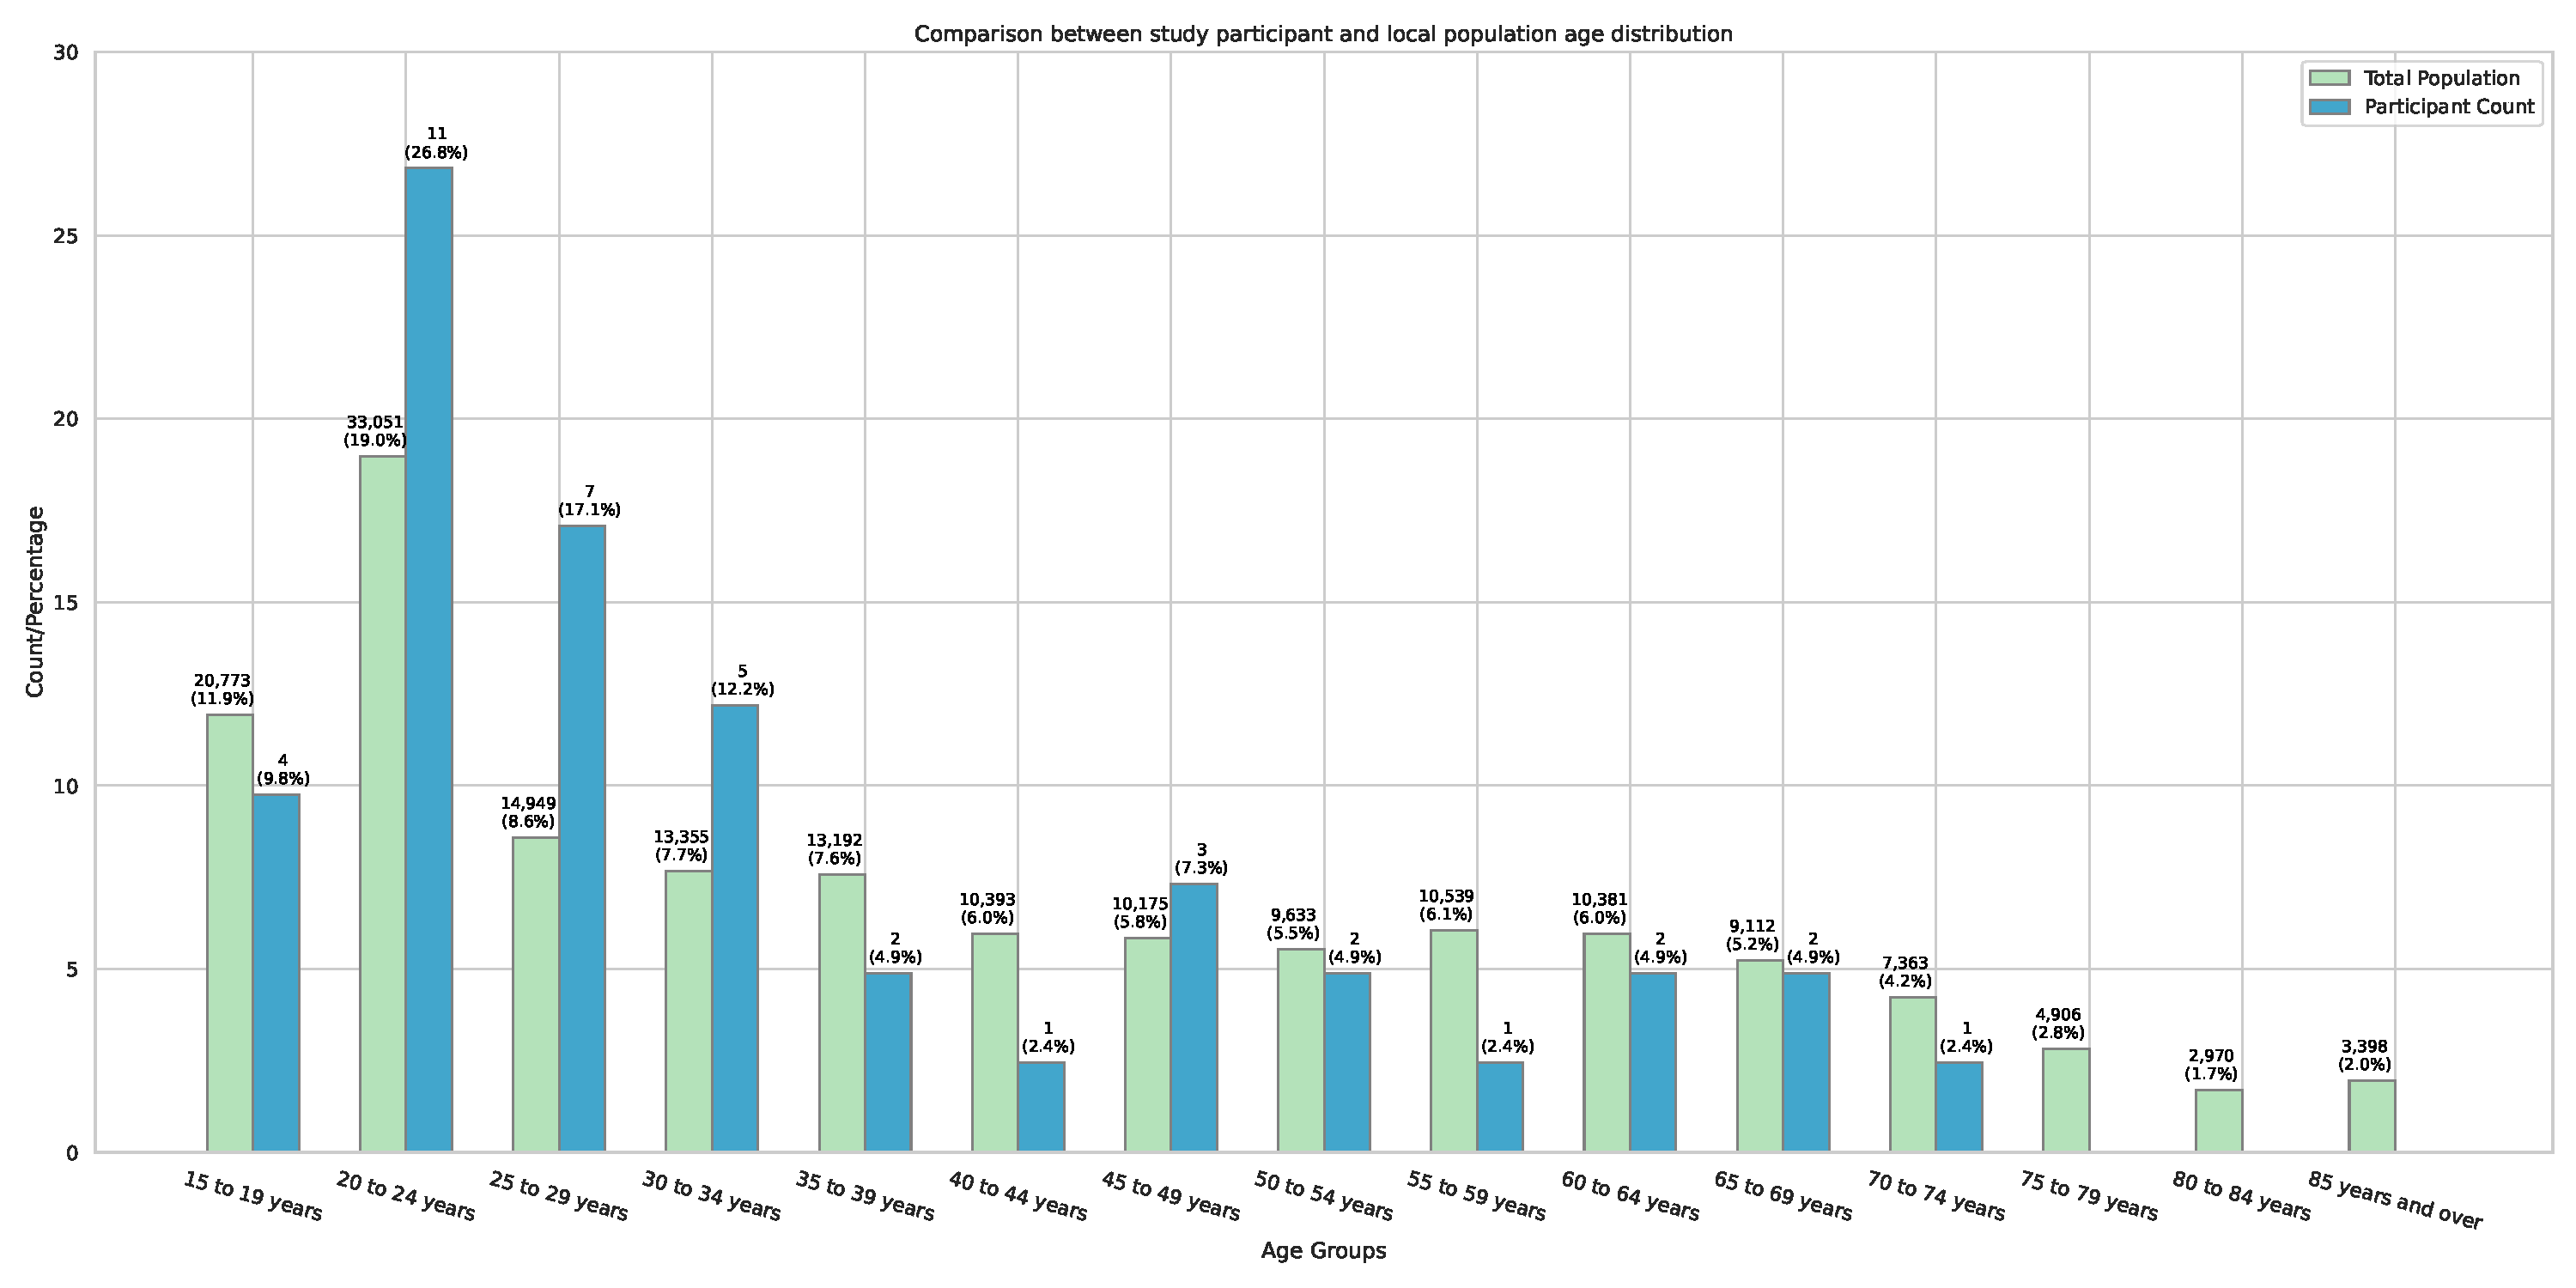
\includegraphics[width=\textwidth]{content/image/demo/demo_age_group_vertical.pdf}
        \caption{Age distribution}
        \label{fig:demoAge}
    \end{subfigure}
    
    \vspace{0.5cm} % Add some vertical space between the rows

    % Bottom figures
    \begin{subfigure}[b]{0.45\textwidth}
        \centering
        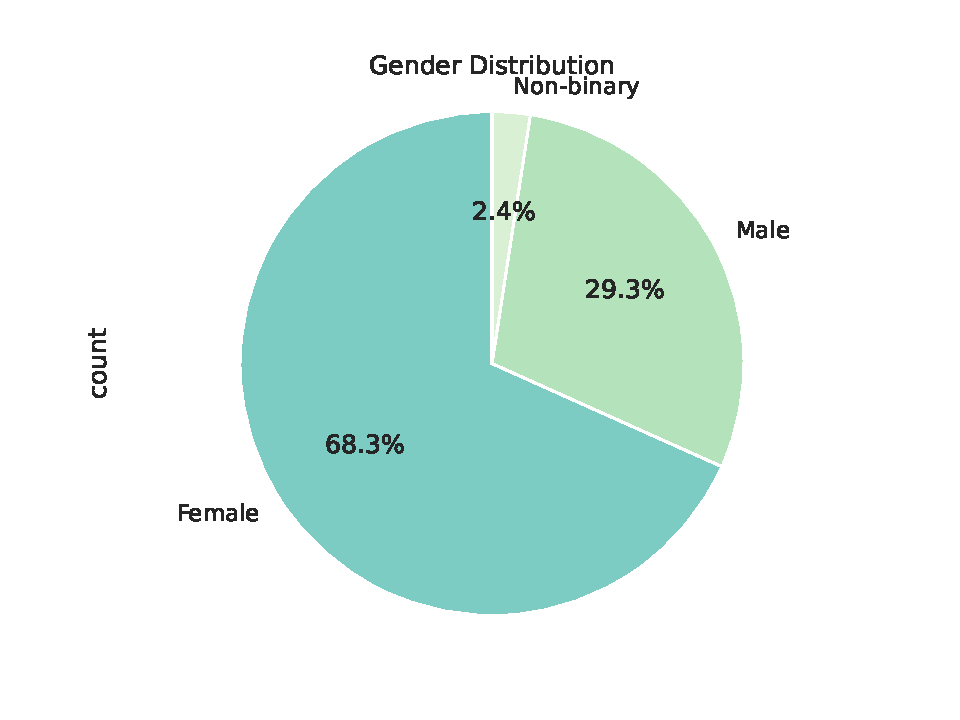
\includegraphics[width=\textwidth]{content/image/demo/demo_gender.pdf}
        \caption{Gender distribution}
        \label{fig:demoGender}
    \end{subfigure}
    \hfill
    \begin{subfigure}[b]{0.45\textwidth}
        \centering
        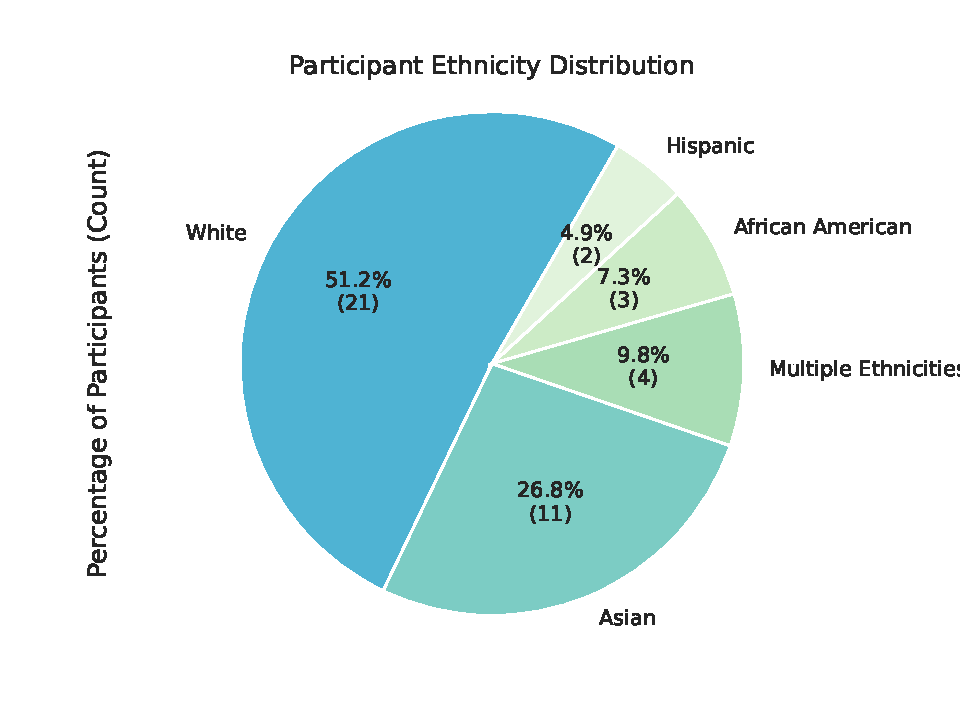
\includegraphics[width=\textwidth]{content/image/demo/demo_ethnicity.pdf}
        \caption{Ethnicity distribution}
        \label{fig:demoEthnicity}
    \end{subfigure}
    
    \caption{Demographic distributions: Age, Gender, and Ethnicity}
    \label{fig:Demographics}
\end{figure}

% maybe more the figure to the appendix?
\section{Cognitive Load and Sources across Experiment Conditions}
\label{sec:cog_result}
In this section, we present the cognitive load across experiment groups and the sources contributing to each cognitive load dimension. Given the limited number of participants, we focus on descriptive statistics and qualitative assessments of cognitive load. Quantitative data includes metrics from the survey tasks, while qualitative insights come from post-survey interviews transcribed and analyzed by the first author.

To analyze the qualitative data, the first author conducted an inductive thematic analysis process~\cite{olsonWaysKnowingHCI2014}. They coded snippets from each transcript based on specific research questions and topics of interest for the qualitative analysis. Similar codes were merged within each research question or topic to form relevant themes. When differences were hypothesized, they applied a deductive coding process to text snippets related to a specific research question or topic of interest.

The results for this section are organized as follows: We start with participant demographics and then provide an overview of our cognitive load findings. We then examine the six dimensions used in the NASA-TLX survey: mental demand, physical demand, temporal demand, performance, effort, and frustration.

\subsection{Demographics}
We recruited a total of $41$ participants, allocating ten to each experiment condition. Due to data quality concerns, we excluded one participant's data\footnote{The participant reported that they did not complete the survey seriously since they think the experiment is fake.}. The mean age of the participants was $34.63$ years old, with a detailed age distribution presented alongside the county population distribution in Figure~\ref{fig:demoAge}. This comparison reveals that our sample closely matches the county's demographic profile, albeit with a slightly higher representation of younger adults, particularly in the 35-45 age range. As shown in Figure~\ref{fig:demoGender}, the majority of participants skewed toward females.

Regarding ethnicity, $51.2\%$ of the participants identified as White, $26.8\%$ as Asian, $7.3\%$ as African American, and $4.9\%$ as Hispanic. Additionally, $9.8\%$ of participants reported mixed ethnicity.

\subsection{Overall Cognitive Load}
\label{sec:cog}
\begin{figure}[ht]
    \centering
    \begin{subfigure}[b]{0.45\textwidth}
        \centering
        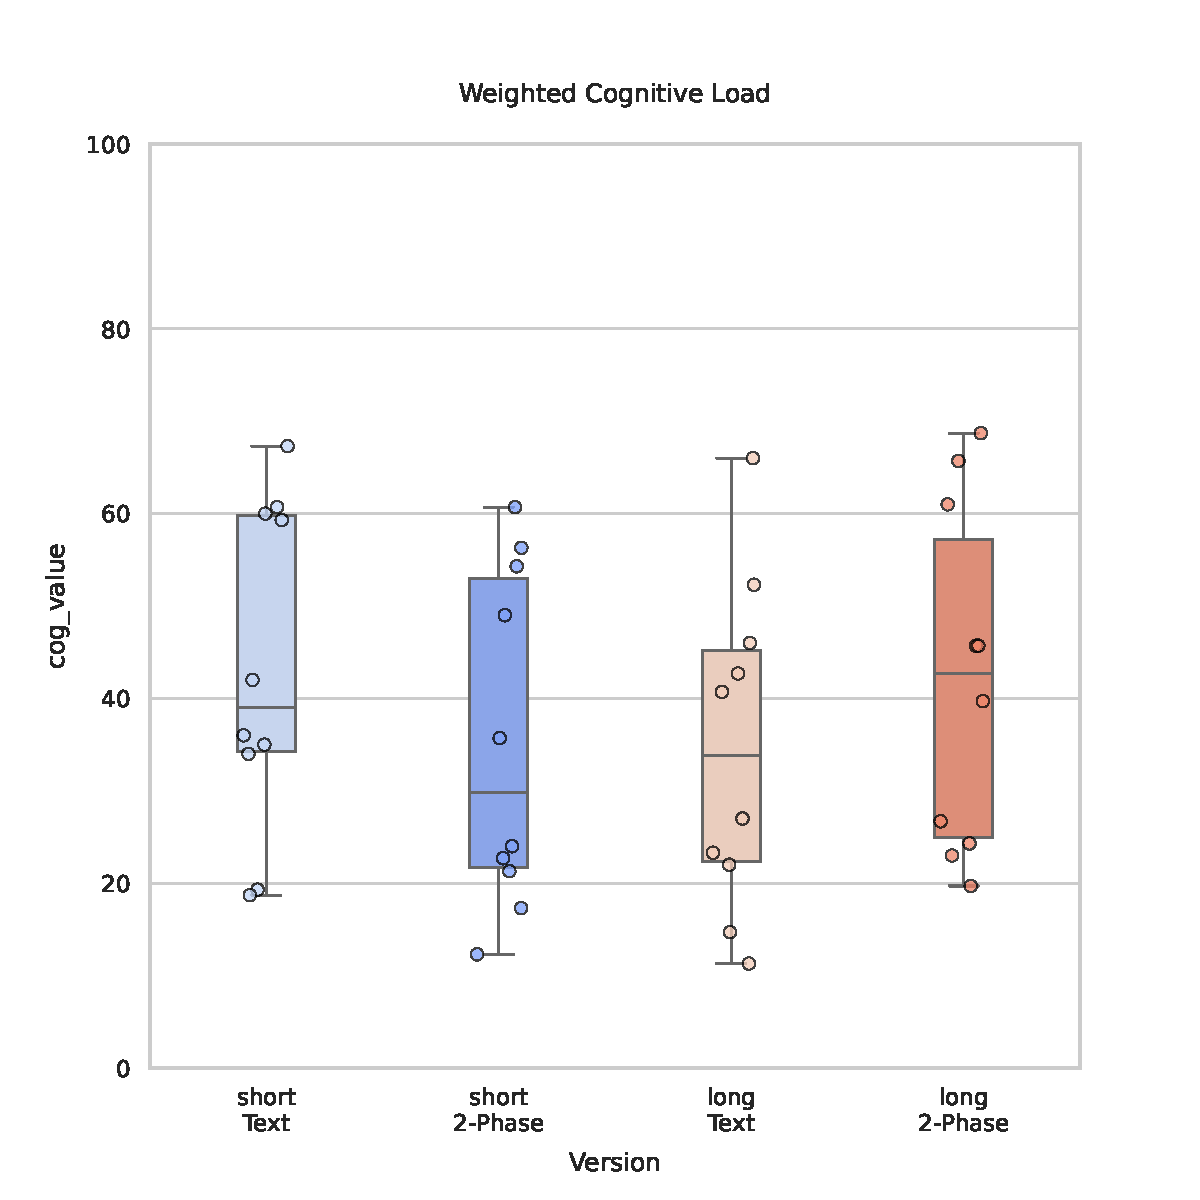
\includegraphics[width=\textwidth]{content/image/results/nasatlx_final_value.pdf}
        \caption{NASA-TLX Weight Score: The Long Two-Phase Interface exhibits the highest weighted cognitive load with a median of $42.70$, a mean of $42.02$. This is higher than the Long Text Interface, which has a median cognitive load of $33.85$, a mean of $34.60$. However, the Short Text Interface demonstrates a higher cognitive load with a median of $39.00$, a mean of $43.23$, compared to the Short Two-Phase Interface which has a median of $29.85$, a mean of $35.36$. Standard deviation are similar across groups at around $18$.}
        \label{fig:nasatlx-final1}
    \end{subfigure}
    \hfill
    \begin{subfigure}[b]{0.47\textwidth}
        \centering
        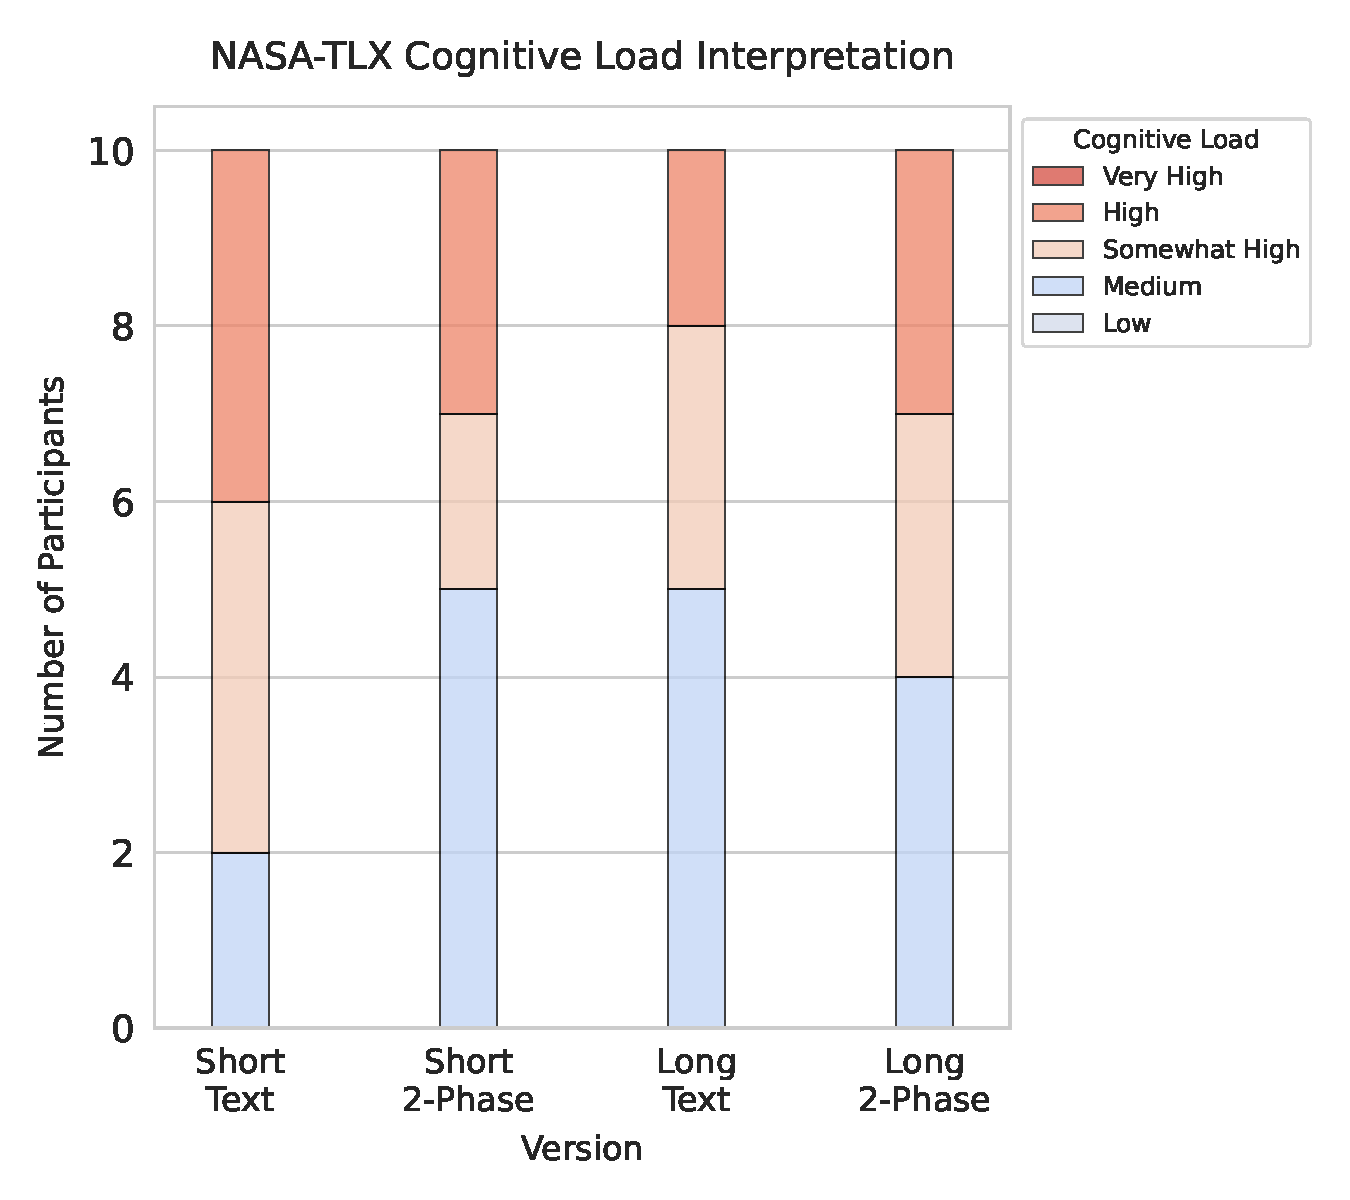
\includegraphics[width=\textwidth]{content/image/results/nasatlx_cog_value_interpreted.pdf}
        \caption{NASA-TLX Cognitive Interpretation: More participants in the Short Text Interface, totaling $8$, reported a somewhat high or above cognitive load, which is significantly higher compared to the $5$ participants who reported similarly for the Short Two-Phase Interface. However, the Long Two-Phase Interface saw slightly more participants, $6$ in total, reporting somewhat high or above cognitive load compared to the Long Text Interface.\vspace{21pt}}
        \label{fig:nasatlx-final2}
    \end{subfigure}
    \caption{This figure shows the box plot results for weighted NASA-TLX scores across experiment groups and participant counts based on individual score interpretations. In~\ref{fig:nasatlx-final1}, we observe a downward trend in cognitive load for the short QS, while the long QS shows an upward trend. Interestingly, there is a counterintuitive downward trend between short and long text interfaces. In~\ref{fig:nasatlx-final2}, these trends are clearer when NASA-TLX scores are grouped into five tiers.}
    \label{fig:nasatlx-final}
\end{figure}

To answer~\textbf{RQ1} and~\textbf{RQ2a}, we derive the weighted NASA-TLX scores across the four experiment conditions. We show these results in Figure~\ref{fig:nasatlx-final}. Weighted NASA-TLX uses a continuous 0-100 score, with higher values indicating greater cognitive load. We use predefined mappings of NASA-TLX values to cognitive levels: low, medium, somewhat high, high, and very high, as listed by~\textcite{hart1988development}. We show value interpretations in Figure~\ref{fig:nasatlx-final2}. 
% We provide summary statistics of the scores here as well:

% \begin{itemize}
%     \item Short text interface: The median cognitive load was $39.00$, with a mean of $43.23$ and a standard deviation of $17.65$. $8$ participants reported somewhat high or above, with $4$ reporting high cognitive load.
%     \item Short two-phase interface: The median cognitive load was $29.85$, with a mean of $35.36$ and a standard deviation of $18.17$. $5$ participants reported somewhat high or above, with $3$ reporting high cognitive load.
%     \item Long text interface: The median cognitive load was $33.85$, with a mean of $34.60$ and a standard deviation of $17.69$. $5$ participants reported somewhat high or above, with $2$ reporting high cognitive load.
%     \item Long two-phase interface: The median cognitive load was $42.70$, with a mean of $42.02$ and a standard deviation of $18.48$. $6$ participants reported somewhat high or above, with $3$ reporting high cognitive load.
% \end{itemize}

Surprisingly, cognitive load scores were lower for the long interface than the short interface. Further, the two-phase interface decreased cognitive load compared to the text interface for the short survey but increased it for the long survey. This is evident from the median cognitive load decrease from $39.00$ to $29.85$, with more participants reporting lower cognitive load using the two-phase interface. The short text interface had the most participants ($N=8$) rating their cognitive load as somewhat high or above. The other three conditions had similar distributions, with about half experiencing medium and half somewhat high or high loads.

We acknowledge the possibility that the elicited values are pure noise and do not reflect the actual cognitive load. This could be due to the small sample size, the nature of the task, or the participants' understanding of the cognitive load scale. However, to dig deeper into this phenomenon, we turn to qualitative insights from the post task interviews.

%By deduction, if the two-phase interface increased cognitive load in the long survey, we might expect a similar increase in the short two-phase interface compared to the short text interface. However, we observed a lower cognitive load in the short two-phase interface. This discrepancy suggests two plausible explanations:

%\paragraph{Two-phase interface prevents satisficing from cognitive overload} The long survey leads to cognitive overload and encouragesd satisficing behaviors, but the interactive components may have prevented participants from taking these mental shortcuts, which would typically reduce measured cognitive load~\cite{daniel2017thinking, simonBehavioralModelRational1955, payneAdaptiveStrategySelection1988, tverskyJudgmentsRepresentativeness}. This prevention could result in a higher cognitive load in the long two-phase interface compared to the long text interface. In other words, the two-phase interface may have shifted participants' cognitive load from some dimensions to others, maintaining their overall cognitive load at a higher level but not overloaded. If this is true, we expect to see differences among the qualitative explanations of sources, specifically differences in the perceived causes of cognitive load. We will explore this in the next subsections (Subsections~\ref{sec:mental}-\ref{sec:fustration}).

%\paragraph{A Pure Increase of Cognitive Load Due to Interactivity} It is also possible that the long survey introduced statisficing behaviors due to cognitive overload, and the two-phase interface did not influence participants' preference construction but only increased cognitive load due to the added interactivity. In other words, participants are asked to perform additional operations with interactive elements that contribute to a higher cognitive load without providing sufficient cognitive benefits. If this is true, we should expect behavior data to show similar voting patterns across conditions, as the added interactions primarily focused on the pre-organization of the options rather than influencing the decision-making process itself. We will explore this in the section~\ref{sec:behave_result}.

%We also acknowledge the possibility that the elicited values are pure noise and do not reflect the actual cognitive load. This could be due to the small sample size, the nature of the task, or the participants' understanding of the cognitive load scale. While this might be true for small sample sizes, we believe that the qualitative insights from the interviews provide a more nuanced understanding of the cognitive load sources. We detail these limitations in Section~\ref{sec:limitations}.

% ============================================= %
\subsection{Sources of Mental Demand}
\label{sec:mental}

%\vspace{5pt}
\begin{tldrbox}
   \faKey~\textbf{Key Differences:} First, slightly more participants using the text interface reported mental demand from precisely determining the number of votes for options compared to the two-phase interface. Second, when it comes to long QS, participants using the long two-phase interface considered broader societal impacts and evaluated options holistically, while those in the long text interface focused on personal relevance and individual issues. % These differences indicate that the two-phase interface encouraged deeper thinking, shifting the source of mental demand. % We find evidence that the two-phase interface prevented cognitive overload.
\end{tldrbox}

Mental demand refers to the degree of mental and perceptual activity required to complete a task. Interview results showed primary drivers of participants' mental demand were~\textit{Budget management} and~\textit{Preference construction}~\footnote{The full table is in Appendix~\ref{apdx:mental_table}.}. %Table~\ref{tbl:mental} listed all causes.

\subsubsection{Mental Demand Source \#1: Budget management} $14$ participants expressed demand from budgeting within limited credit (\smallquote{S032}{~\bracketellipsis in order to like show your support for certain societal issues you had to~\ldots take away from other societal issues that you could support.}, $N=5$), tracking remaining credits (\smallquote{S006}{~\bracketellipsis looking at the remaining credits, I'm trying to mentally divide that up before I start allocating}, $N=10$), and maximizing credit use (\smallquote{S032}{I just wanted to make sure that I used all the credit that I had available to me}, $N=8$).

We further categorized budget management-induced mental demand as either operational (corresponding to a single interface-level action, e.g., using the last remaining credit) or strategic (achieving a higher-level goal, e.g., evenly distributing credits across options).  We noticed that long survey participants tended to report operational causes of mental demand rather than strategic ones, which may indicate that the larger number of survey options induced more short-term thinking.

\subsubsection{Mental Demand Source \#2: Preference construction}
All but one participant reported increased mental demand due to preference construction. We further break it down into three sources: comparative preference evaluation (i.e., evaluating relative importance between options; \smallquote{S002}{Figuring out \dots how much I prioritize option 1 over option 2}, $N=16$), resource-constraint prioritization (i.e., trading off between options due to resource constraints, \smallquote{S005}{~\bracketellipsis was very hard to take decisions~\ldots because I felt that multiple options deserve equal amount of credit~\ldots but you have given very limited amount of credit.}, $N=17$), and precise resource allocation (\smallquote{S023}{~\bracketellipsis having to pick how many upvotes would go to each one}, $N=30$).

Almost all participants mentioned preference construction as a source of mental demand, supporting the theory that preference construction is a difficult and mentally demanding task. Notably, more participants using the text interface reported mental demand from precise resource allocation compared to the two-phase interface ($18$ vs. $12$). We conjecture that the first pass on the survey items in the organization phase helped participants reduce their mental demands in this area once they got around to vote allocation.

In addition, when categorizing preference construction-induced mental demand, participants ($N=8$) in the long text interface tend to consider a smaller scope that focuses on personal relevance. Conversely, participants ($N=9$) in the long two-phase interface considered the broader societal impact and evaluated options more comprehensively. Compare the following two quotes, where one focused on adjusting credits between two options and the other reflecting across broader societal values:

\begin{displayquote}
Trying to figure out what upvotes I should give~\bracketellipsis I kind of went back and forth between those two. \bracketellipsis So it was very mentally tasking for me. \hfill\quoteby{S015 (LT)}
\end{displayquote}

\begin{displayquote}
\bracketellipsis really having to think, especially with so many different societal issues. How do I personally prioritize them? And to what extent do I prioritize them? \hfill\quoteby{S009 (LI)}
\end{displayquote}

Inspecting both causes, while we did not notice significant differences in mental demand raw values (Figure~\ref{fig:mental_cog_score}) across the four experiment groups, especially between the interfaces across long QS, they exhibited different sources contributing to their mental demand.

% Discussion: We argue the two-phase interface prevented participants from using heuristics to narrow their choices, which only appeared when final votes were determined, an area with less support from the interface. We conclude the two-phase interface scaffolded the decision-making process, preventing satisficing behaviors because of cognitive overload, and thus shifted mental demand sources. This shift explains why .


\begin{figure}[h]
    \begin{minipage}[t]{0.45\textwidth}
        \centering
        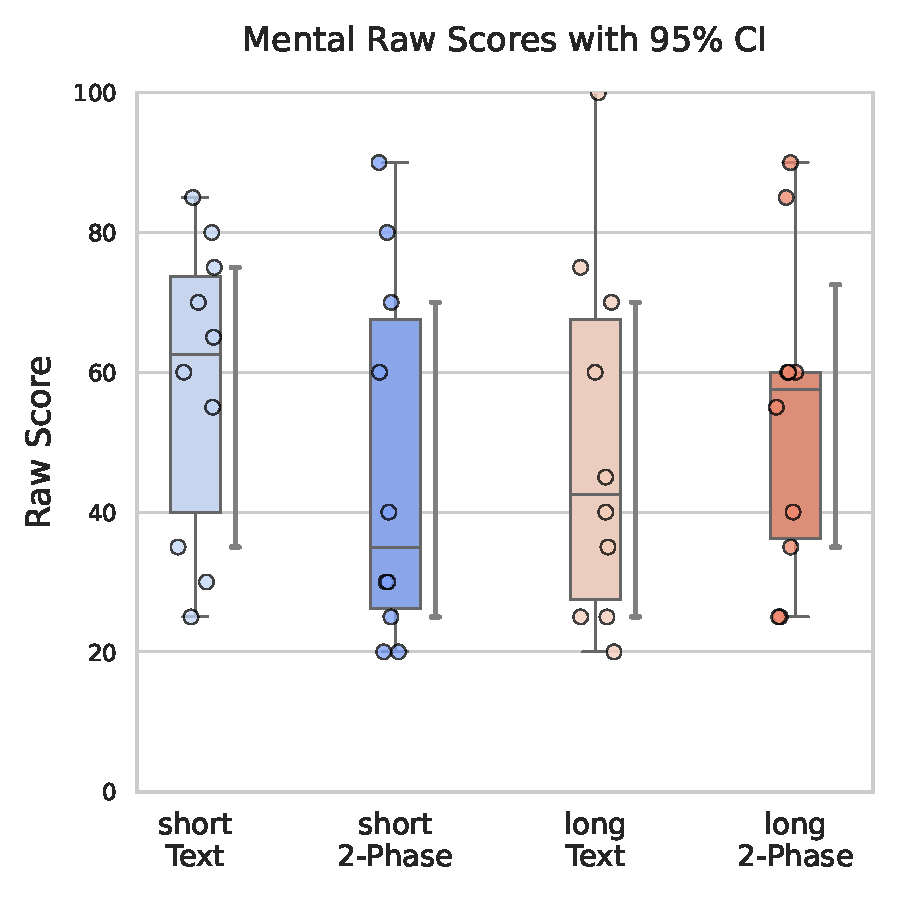
\includegraphics[width=\textwidth, trim=0 13 0 13, clip]{content/image/cog/Mental_scores.pdf}
        \captionsetup{width=0.9\textwidth, justification=justified}
        \caption{Mental Demand Raw Score: Across all four experiment groups, participants' reported mental demand is spread across a wide range with many participants experiencing high mental demand.}
        \label{fig:mental_cog_score}
    \end{minipage}
    \hfill
    \begin{minipage}[t]{0.45\textwidth}
        \centering
        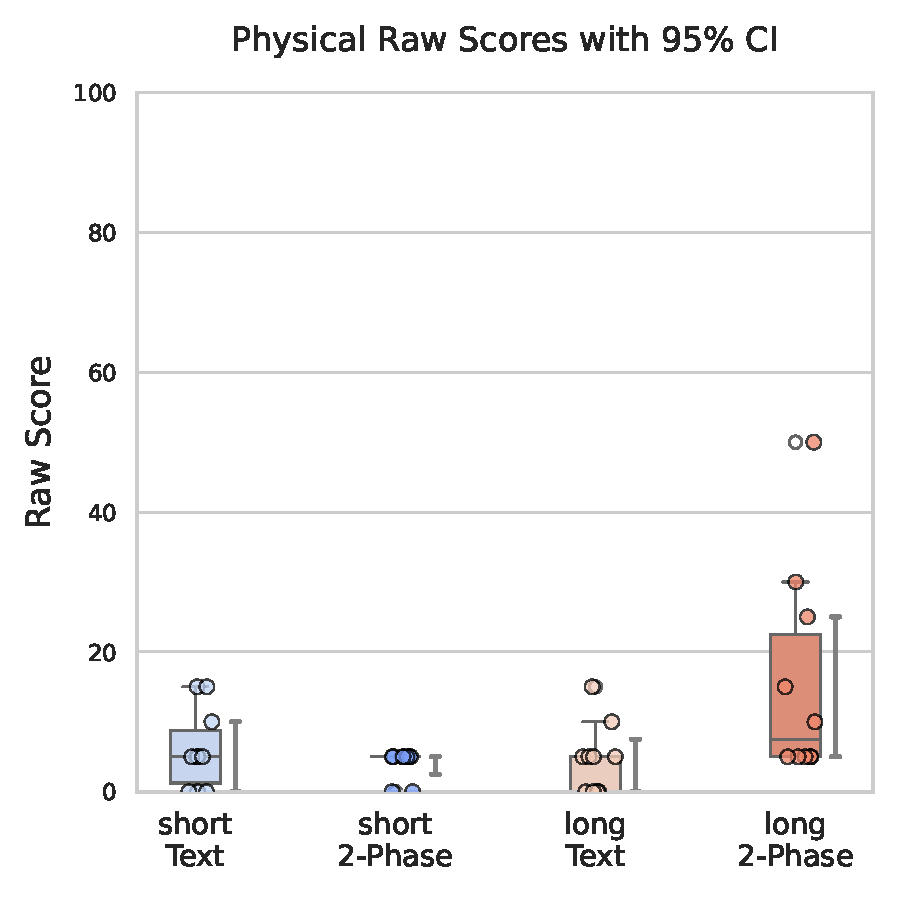
\includegraphics[width=\textwidth, trim=0 13 0 13, clip]{content/image/cog/Physical_scores.pdf}
        \captionsetup{width=0.9\textwidth, justification=justified}
        \caption{Physical Demand Raw Score: Participants other than the long two-phase interface reported minimal physical demand. The long two-phase interface had the highest physical demand, likely due to increased mouse clicks and extended time spent looking at the vertical screen.}
        \label{fig:physical_cog_score}
    \end{minipage}
\end{figure}

% ============================================= %
\subsection{Sources of Physical Demand} 
\label{sec:physical}

%\vspace{5pt}
\begin{tldrbox}
   \faKey~\textbf{Key Differences:} Two-phase interface experienced higher physical demand from increased mouse usage.
\end{tldrbox}

Physical demand refers to the physical effort required to complete a task, such as physical exertion or movement. Since this study involves participants sitting in front of a computer screen completing a survey, most participants reported minimal physical demand($N=32$). We nonetheless report the sources of this minimal demand, which include reading text on the screen ($N=4$), using the mouse ($N=16$), and moving their head to navigate the vertical screen ($N=5$)~\footnote{The full table showing the distribution is in Appendix~\ref{apdx:physical_table}}. Participants emphasized that these demands were minimal, which is reflected in the low values reported in the NASA-TLX physical demand scores (Figure~\ref{fig:physical_cog_score}) Notably, $11$ out of $20$ participants who used the two-phase interface mentioned physical demand from using the mouse, reflecting their increased interaction with the interface. This is further supported by the raw NASA-TLX physical demand scores (Figure~\ref{fig:physical_cog_score}), which show a significant visual difference between short and long two-phase interfaces as well as between text and two-phase interfaces in long surveys.

% ============================================= %
\subsection{Sources of Temporal Demand} 
\label{sec:temporal}

\begin{tldrbox}
   \faKey~\textbf{Key Differences:} % Participants faced increased temporal demand from: \textit{Budget}, \textit{Decision Complexity}, and \textit{Operational Tasks}. The two-phase interface managed temporal demand more effectively, allowing participants to pace themselves and avoid misperceiving task difficulty.
    First, participants using the short text interface wanted to complete the task quickly and reported the highest mental demand. Second, half of the participants using the long two-phase interface acknowledged making decisions, which caused some mental demands. Last, participants using the long text interface showed the lowest temporal demand score.
\end{tldrbox}

\begin{wrapfigure}{r}{0.45\textwidth} % Adjust the width as needed
    \centering
    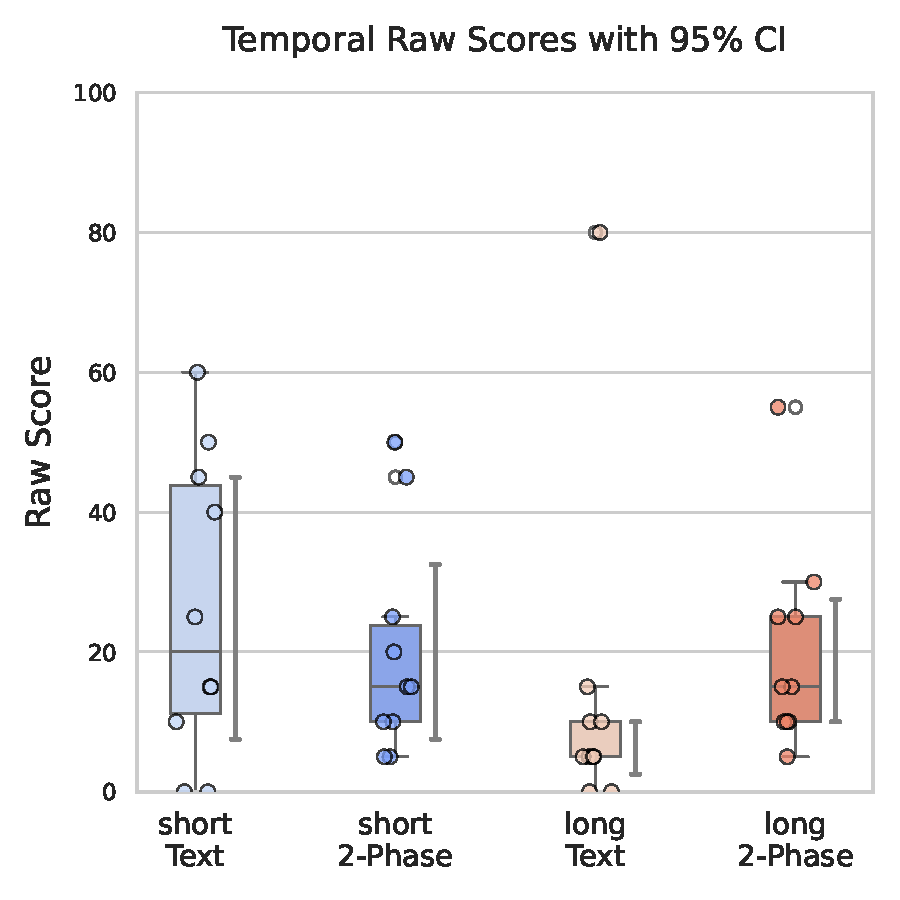
\includegraphics[width=0.45\textwidth, trim=0 13 0 13, clip]{content/image/cog/Temporal_scores.pdf}
    \captionsetup{width=0.45\textwidth, justification=justified} % Adjust the width to match the image width
    \caption{Temporal Demand Raw Score: The short text interface results in the highest temporal demand, while the long text interface is the lowest. Two-phase interfaces, show moderate temporal demand, suggesting that interactive elements allowed participants to pace themselves better.}
    \label{fig:temporal_cog_score}
\end{wrapfigure}

Temporal demand measures the time pressure participants feel during a task. Lower demand indicates participants felt comfortable taking a more leisurely pace. We categorize the main sources of increased temporal demand as stemming from  ~\textit{Decision Complexity} and ~\textit{Operational Tasks}  (Table~\ref{tbl:temporal}). \textit{Budget} also came up occasionally (\smallquote{S034}{as the money decreases I felt kind of rushed}, $N=4$).


\subsubsection{Temporal Demand Source \#1: Decision Quantity}
Participants often felt there were too many decisions to make. We observe no significant difference in how often participants expressed concerns about temporal demand across conditions. However, how they expressed their concerns differed. These concerns were either expressed affirmatively or negatively. Affirmative expression refers to cases where participants stated there were too many remaining decisions to make (\smallquote{S022}{So it didn't take too much time. but obviously there was a lot of things to consider, so there was some temporal demand.}), while negative expression refers to participants' concerns regarding the time and effort already invested (\smallquote{S024}{maybe I should just hurry up and make a decision.}). Five participants from the short text interface expressed negative perceptions of temporal demand and no participants expressed concerns affirmatively. In contrast, five participants from the long two-phase interface expressed affirmatively with zero negatively.

\subsubsection{Temporal Demand Source \#2: Operational Tasks}
Lower-level operational tasks were also often discussed as sources of temporal demand. Operational tasks involve actions like updating votes and completing the survey. For instance, one participant aimed to operate swiftly:

\begin{displayquote}
I wanna get through things in an efficient manner which doesn't necessarily mean I rush it. But it does mean that I do things expeditiously. Especially. I'd like to think I'm somewhat computer-savvy. And so to be able to move through this quickly and efficiently. I do take pride in it, but it's all personal stuff. It's not nothing outwardly influencing me. 
        
\noindent \hfill -- S032, short text interface
\end{displayquote}

The raw NASA-TLX values in Fig~\ref{fig:temporal_cog_score} first highlighted that temporal demand trended lower for the two-phase interface in the short QS condition while it trended higher for the long QS condition. Second, the long text interface exhibited the lowest temporal demand, which is counter intuitive since participants in this condition made no fewer decisions and operations compared to the short text group. Although we were initially surprised to find that temporal demand was higher for the short survey experiment group, we noticed that more participants who experienced a short survey expressed a desire to complete the task quickly. Over half of the participants from the short interface wanted to complete the task swiftly and quickly, compared to $5$ participants from the long QS group. Thus, our counter-intuitive findings around temporal demand may be explained by the fact that participants who received the short survey had higher expectations to complete the survey swiftly.

%\subsubsection{Takeaway: Temporal demand managed through two-phase interface}
%The raw NASA-TLX values in Fig~\ref{fig:temporal_cog_score} visually indicate two important points. First, temporal demand trended lower for the two-phase interface in the short QS condition, while it trended higher for the long QS condition. Second, the long text interface exhibited the lowest temporal demand, which is counterintuitive since participants in this condition made no fewer decisions and operations compared to the short text group. According to our interpretation of mental demand results in Section~\ref{sec:mental_takeaway}, participants likely did not experience temporal demand because they applied heuristics to reduce the number of decisions, thereby lowering their cognitive load and decision-making instances.

%Additionally, participants in the long interactive condition reported that the numerous required operations created temporal demand, preventing them from taking mental shortcuts and shifting their cognitive load to different dimensions.

%Furthermore, participants in the short text QS expressed high temporal demand and perceived it negatively, likely misperceiving task difficulty. Conversely, even though the short two-phase interface required more decisions, participants reported less temporal demand from decision-making, resulting in a lower overall score. This suggests that the two-phase interface slowed them down without increasing temporal demand, allowing them to pace themselves and engage in more in-depth thinking, thereby preventing a misperception of task difficulty.

%These observations across experimental conditions support the plausible explanation that the two-phase interface mitigated satisficing behaviors due to cognitive overload, as evidenced by the different sources of temporal demand.

%  TODO: move to discussion?
% It is also worth noting that three participants from the 20 who responded to the long survey mentioned that the vertical screen's ability to see all options facilitated direct comparisons and transparency about the entirety of the task, which reduced the temporal demand.

% \begin{displayquote}
% (Seeing) all at once I can see how many there are, so it's kind of like I can kind of tell when I will be done.

% \noindent \hfill -- S041, long text interface
% \end{displayquote}

% ============================================= %
\subsection{Source of Performance}
\label{sec:performance}
%\vspace{5pt}

\begin{tldrbox}
   \faKey~\textbf{Key Differences:} Participants who used a two-phase interface were generally more positive about their final outcome -- they were twice as likely to report "feeling good" about their final results
 % Participants experienced performance demands due to \textit{Operational Actions} and \textit{Social Responsibility}. Despite similar performance scores across groups, more participants using the two-phase interface felt more positive about their performance.
\end{tldrbox}

Performance refers to a person's perception of their success in completing a task. Lower values mean good perceived performance; higher values mean poor perceived performance. We found minimal qualitative differences between experiment groups regarding factors influencing perceived performance. Two influencing factors arose from the interviews: \textit{Operational Actions} and \textit{Social Responsibility}~\footnote{The full performance table is at Appendix~\ref{apdx:perf_table}}. Despite most participants reporting positively on their performance, nuances exist in how different groups interpret their performance.

\subsubsection{Operational Actions}
Operational actions, like the theme presented in temporal demand, refer to specific, executable procedures participants perform in the survey. This could involve: pressure to spend all credits or stay within budget ($N=6$), fears that final vote choices did not reflect true preferences($N=5$), or concerns that they had finished the task inefficiently ($N=6$).

\subsubsection{Social Responsibility}
Social responsibility-based concerns around performance came up when participants reflected on how their final vote counts would be perceived by others (\smallquote{S041}{I don't want people to think that I just like don't care about <ethnicity> people at all}) or influence real-world decision-making (\smallquote{S027}{Some of these things might \ldots have outcomes that I didn't foresee}).

All groups cited social responsibility as source to evaluate effort. Raw NASA-TLX scores (Figure~\ref{fig:performance_cog_score}) show participants had indistinguishable performance scores. This aligns with the interview results where most participants felt positive about their final submission. 

To dig deeper, we also analyzed participants' language when they described their performance. Expressions like ``good enough'' may be indicative of satisficing behaviors -- our results suggest participants are satisfied at similar rates regardless of the interface. 1/4 of the participants in the text interface expressed ``done their best,'' referring to exhausting their effort. Participants who used a two-phase interface were generally more positive about their final outcome -- they were twice as likely to report "feeling good" about their final results ($N=11$ vs $N=6$).

% TODO: Need to check the reflective thinking part a bit. I **think** there are differences but it is unclear, need to go back to raw code.

\begin{figure}[h]
    \begin{minipage}[t]{0.45\textwidth}
        \centering
        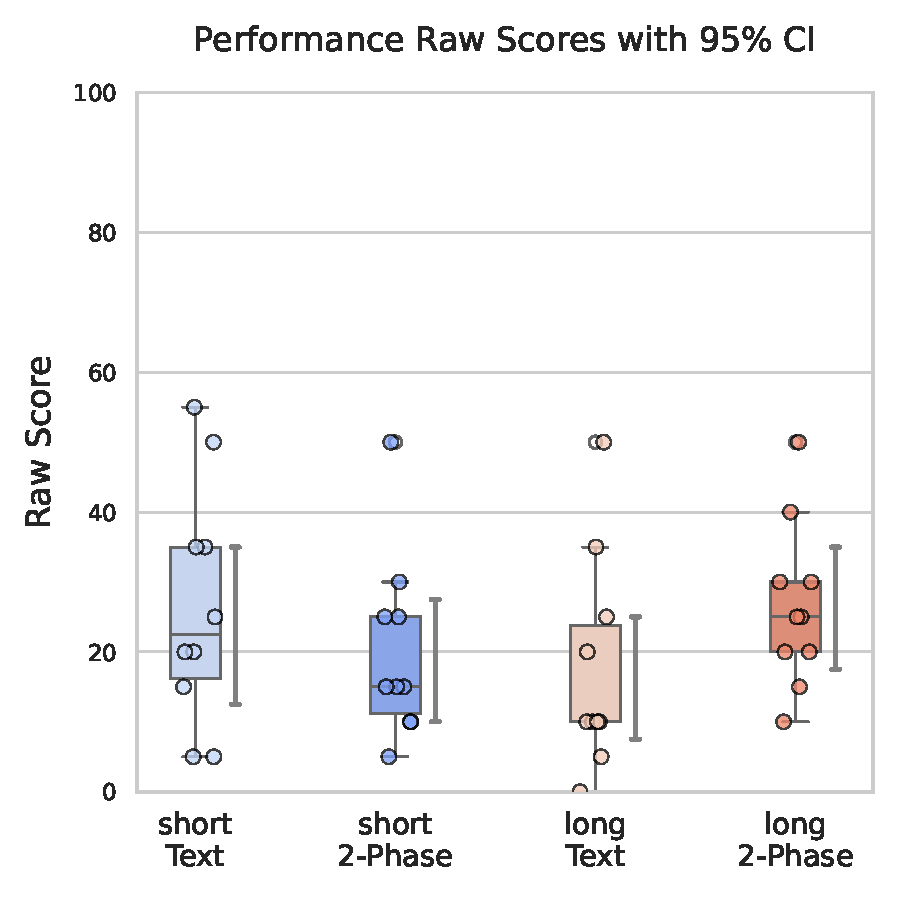
\includegraphics[width=\textwidth, trim=0 13 0 13, clip]{content/image/cog/Performance_scores.pdf}
        \captionsetup{width=\textwidth, justification=justified} % Adjust the width to match the image width
        \caption{Performance Demand Raw Score: Participants showed indifferent performance raw scores across experiment conditions, all trending toward satisfactory.}
        \label{fig:performance_cog_score}
    \end{minipage}
    \hfill
    \begin{minipage}[t]{0.45\textwidth}
       \centering
       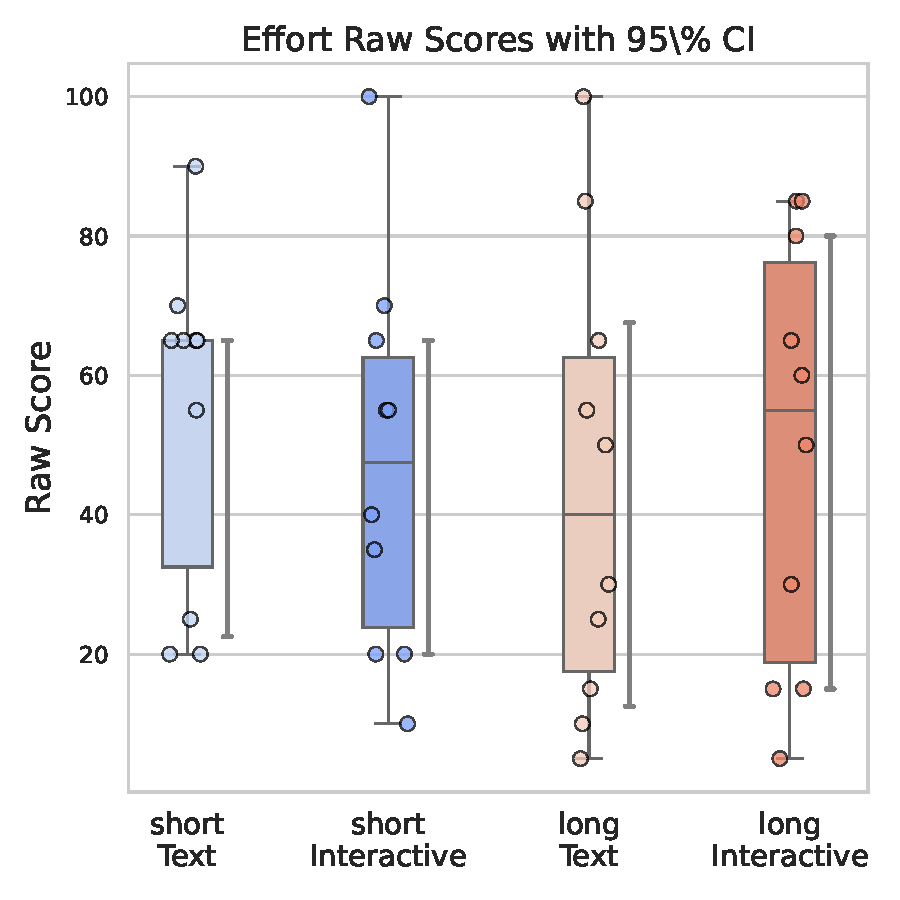
\includegraphics[width=\textwidth, trim=0 13 0 13, clip]{content/image/cog/Effort_scores.pdf}
       \captionsetup{width=\textwidth, justification=justified} % Adjust the width to match the image width
       \caption{Effort Raw Score: Effort scores show indifference across groups.}
       \label{fig:effort_cog_score}
    \end{minipage}
\end{figure}


% ============================================= %
\begin{table}[h]
    \caption{Effort Sources: Participants using the text interface focused more on operational tasks, while those using the two-phase interface focused more on strategic planning.}
    \label{tbl:physical}
    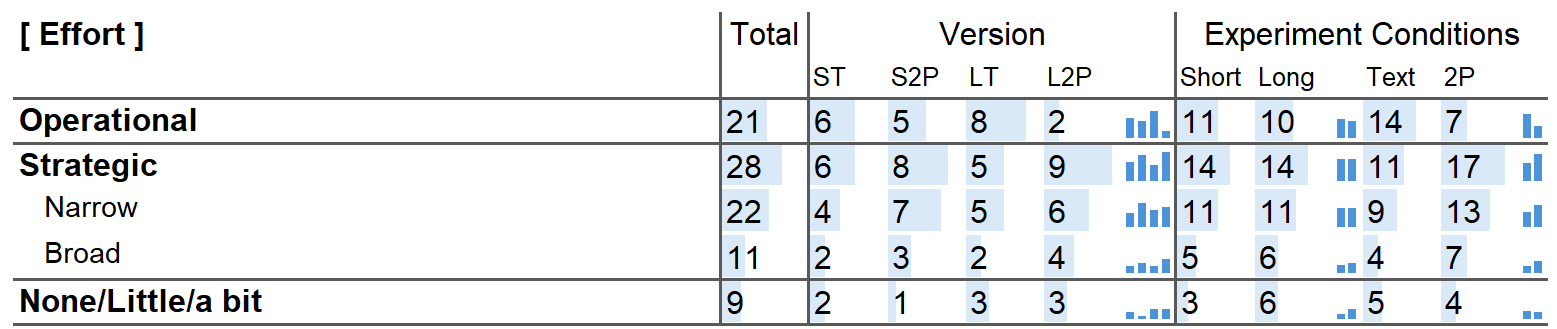
\includegraphics[width=\linewidth]{content/image/cog/effort_table.png}
\end{table}

\subsection{Source of Effort}
\label{sec:effort}

%\vspace{5pt}
\begin{tldrbox}
   \faKey~\textbf{key Differences:} First, participants in the text interface associated effort with operational tasks more often than participants from the two-phase interface. Conversely, participants in the two-phase interface cited more sources from strategic planning than those in the text interface. We observed that participants experienced effort when considering a comprehensive view while using the interactive interface.
   
   %Effort sources varied between operational~\textit{Operational Tasks} and~\textit{Strategic Planning}. Participants using the text interface focused on operational tasks, while those using the two-phase interface engaged in strategic planning. This shows that the two-phase interface spurs deeper, more critical thinking.
\end{tldrbox}
Effort refers to how hard participants felt they worked to achieve the level of performance they did. Because effort includes the intensity of both mental and physical resources expended during the task, we refer readers to \cref{sec:mental} and \cref{sec:physical} to understand the definitions of these sources.

%We identified two major sources of effort: \textit{Operational Tasks} and \textit{Strategic Planning}.

\subsubsection{Effort Source \#1: Operational Tasks} $14$ of the $20$ participants using the text interface mentioned Operational Tasks as effort sources, compared to $7$ using the two-phase interface, with the lowest mention by the long two-phase interface group ($N=2$). 

\subsubsection{Effort Source \#2: Strategic Planning} Different from Operational Tasks, $11$ participants in the text interface compared to $17$ participants describing strategic planning as sources of effort, with almost all participants ($N=9$) from the long two-phase interface. We further categorize strategic planning into \textit{narrow} and \textit{broad} scopes as we did for mental demand~\cref{sec:mental}. Participants using the two-phase interface ($N=7$) had nearly mentioned double ($N=4$) times regarding global strategies. 

While the raw NASA-TLX effort scores (Figure~\ref{fig:effort_cog_score}) showed a similar spread across experiment groups, akin to mental demand, the qualitative analysis showed more distinction that participants using the two-phase interface considered options more comprehensively and felt less effort on completing operational tasks. 

% However, qualitative analysis revealed that participants using the text interface experienced more effort focused on operational tasks (i.e., completing specific tasks). In contrast, participants using the two-phase interface experienced more effort focused on strategic planning (planning a strategy to complete tasks). Specifically, those using the two-phase interface engaged in global strategic planning, considering options comprehensively and beyond the immediate task. This contrasts with text interface participants, who concentrated more on operational tasks and narrower strategic planning. This finding reinforces that cognitive load sources differ between interfaces, with two-phase interfaces fostering deeper, more critical thinking.

%Both examples show considerations beyond personal experiences, including outcomes or social values. Nearly twice as many participants using the two-phase interface ($N=7$) mentioned global strategic efforts compared to the text interface ($N=4$). Overall, more participants using the two-phase interface ($N=17$) reported sources of strategic effort compared to those using text-based interfaces ($N=11$).

%\subsubsection{Takeaway: Two-phase interface spurs more strategic effort from participants}
%Effort is a realization of mental demand through physical actions. Since participants experienced little physical demand, the sources of effort reflected how individuals translated their mental demand into efforts. The raw NASA-TLX effort scores (Figure~\ref{fig:effort_cog_score}) showed a similar spread across experiment groups, akin to mental demand. However, qualitative analysis revealed that participants using the text interface experienced more effort focused on operational tasks (i.e., completing specific tasks). In contrast, participants using the two-phase interface experienced more effort focused on strategic planning (planning a strategy to complete tasks). Specifically, those using the two-phase interface engaged in global strategic planning, considering options comprehensively and beyond the immediate task. This contrasts with text interface participants, who concentrated more on operational tasks and narrower strategic planning. This finding reinforces that cognitive load sources differ between interfaces, with two-phase interfaces fostering deeper, more critical thinking.

%\begin{displayquote}
%And then I wanted to bump up (an option) maybe to 4 or <option> to 5 and realize I couldn't. My point (number of votes) had to like back down a little bit~\ldots So that would be effort came in of how do I want to really rearrange this to make it (the budget spending) maximize?

%\noindent \hfill -- S029, short text interface
%\end{displayquote}

%\begin{displayquote}
%So it was like it was very~\ldots I have to put a lot of effort in terms of you know~\ldots think about each dimension that if I give one credit to <option name> whether it will affect my credits on <another option name>.

%dent \hfill -- S005, long text interface
%\end{displayquote}

%Both quotes illustrated participants putting in effort to manipulate the interface. .


%\begin{wrapfigure}{r}{0.45\textwidth} % Adjust the width as needed
%    \centering
%    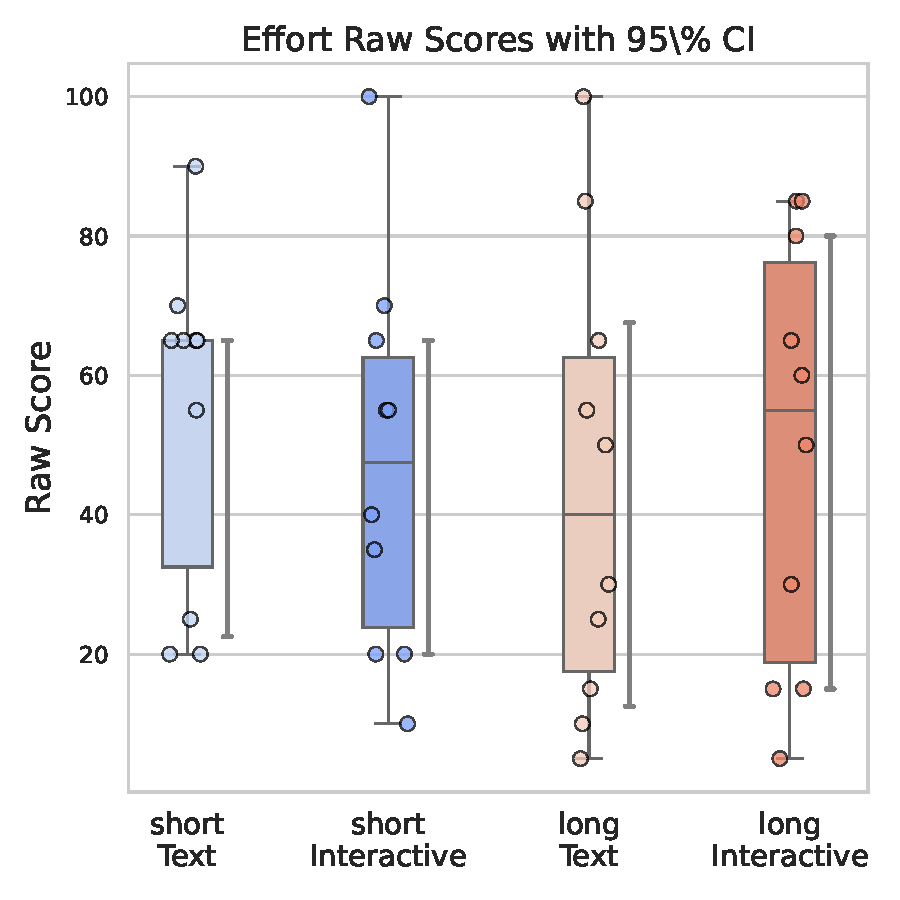
\includegraphics[width=0.45\textwidth, trim=0 13 0 13, clip]{content/image/cog/Effort_scores.pdf}
%    \captionsetup{width=0.40\textwidth, justification=justified} % Adjust the width to match the image width
 %   \caption{Effort Raw Score: Effort scores shows indifference across groups.}
  %  \label{fig:effort_cog_score}
%\end{wrapfigure}


%\subsubsection{Effort Source: Strategic Planning}
%Strategic planning is similar to strategic budget management mentioned under mental demand. Unlike operational tasks, strategic planning involves higher-level strategies to complete the survey. We categorize two distinct types of planning: \textit{personal} and \textit{global}. \textit{Personal strategic planning} involves translating preferences onto the survey without considering broader values or beliefs. For example:

%\begin{displayquote}
%~\bracketellipsis having that prior experience and being able to quickly link it to a tangible thing that I've experienced in my personal life.

%\noindent \hfill -- S032, short text interface
%\end{displayquote}

%\begin{displayquote}
%And really the bulk of the effort was how to rank order these (options) and allocate the resources behind the upvotes so that I can accurately depict what I want~\ldots say, a committee to focus on and allocate actual fungible resources, too. 

%\noindent \hfill -- S019, long two-phase interface
%\end{displayquote}

%Participants using the two-phase interface ($N=13$) mentioned personal strategic planning slightly more than those using the text interface%\end{displayquote}

%\begin{displayquote}
%Hey, even though I don't really like this idea. But what if they're important? They sort of kind of deserve some attention~\ldots that's why I think I have the effort here.

%\noindent \hfill -- S037, long two-phase interface
%\end{displayquote}
    


% ============================================= %
\subsection{Source of Frustration} 
\label{sec:fustration}

%\vspace{5pt}
\begin{tldrbox}
   \faKey~\textbf{Key differences:} We observed evidence that participants in the long text interface showed least amount of frustration from operational causes compared to other experiment conditions.%Participants experienced frustration from two main sources: \textit{Operational Actions} and \textit{Strategic Planning}. We observed evidence that participants in the long text interface showed little frustration, specifically from operational sources, indicating satisficing behaviors.
\end{tldrbox}

Frustration refers to the extent to which the participant is annoyed, irritated, or discouraged during the task. Sources of frustration were generally related to either: \textit{Operational Actions} like credit management ($N=6$) and dealing with the quadratic vote costs ($N=5$), or \textit{Societal Concerns},  like wishing they did not have to make tradeoffs ($N=8$) or feeling pessimistic about how others will vote ($N=6$). We provide the full table in Appendix~\ref{apdx:frus_table}

In general, the frustration derived from societal concerns did not seem strongly affected by any of the experimental conditions. With respect to operational action-driven frustration, however, we saw some discrepancies. The long text interface condition had the fewest participants expressing operational frustration, with half expressing no frustration, mirroring the trends in the actual scores (Figure~\ref{fig: fustration_cog_score}). Prior literature~\cite{polmanWhyAreMaximizers2010, schwartzMaximizingSatisficingHappiness2002} indicates that satisficers tend to be less frustrated and happier than maximizers. Thus, participants in the long text interface exhibit satisficing behaviors, further supporting our claim that the two-phase interface can reduce satisficing behaviors in QS tasks.


%\subsubsection{Operational Actions} 
%$15$ participants highlighted this source for frustration. $6$ participants expressed frustration regarding credit management (i.e., overspending budget); $4$ participants mentioned had trouble deciding the final value for the options; $3$ participants are frustrated because they need to make multiple decisions; $5$ participants were frustrated with the quadratic mechanism; $4$ participants are frustrated trying to understand the content of the option or how the option connects to them. For example, 

%\begin{displayquote}
%I was slightly frustrated when doing the task, probably because there was a budget that we kind of had to stick with it.

%\noindent \hfill -- S001, long text interface, quadratic mechanism
%\end{displayquote}

%\begin{displayquote}
%i think just frustration~\bracketellipsis because when i was making like the decisions on how many upvotes I could put in each section, I was running out of credits.

%\noindent \hfill -- S013, short two-phase interface, budget management
%\end{displayquote}

%These demonstrate participants' frustration when hindered by operational actions or constraints presented by QS. Notably, almost half of the participants in all experiment groups expressed operational frustration, compared to only two participants from the long text interface group.

%\begin{wrapfigure}{r}{0.45\textwidth} % Adjust the width as needed
%    \centering
 %   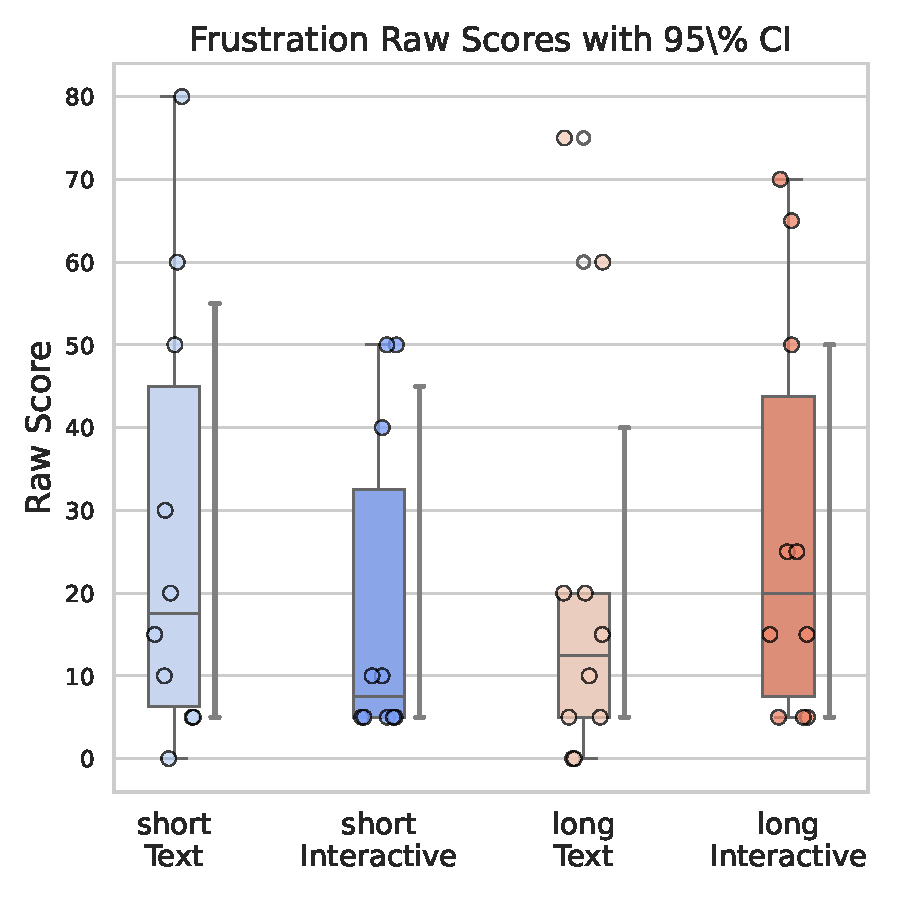
\includegraphics[width=0.45\textwidth, trim=0 13 0 13, clip]{content/image/cog/Frustration_scores.pdf}
 %   \captionsetup{width=0.40\textwidth, justification=justified} % Adjust the width to match the image width
  %  \caption{Fustration Raw Score: Participants other than the long text interface highlighted seversl operational tasks that led to fustration. All groups share causes from strategic planning.}
    %\label{fig:fustration_cog_score}
%\end{wrapfigure}

%\subsubsection{Strategic Planning}
%We derived strategic planning into two types: \textit{lower-level} and \textit{higher-level}. Four participants experienced conflict between their own and others' preferences. Eight participants experienced conflict when making trade-offs among a few options. For example:

%\begin{displayquote}
%Because I know that's important to other people. But it just doesn't to me.
    
%\noindent \hfill -- S010, short two-phase interface
%\end{displayquote}

%\begin{displayquote}
%I would have loved to have given more to other groups~\ldots and I felt stressed like~\bracketellipsis well~\ldots it's a group that you know is still~\ldots you know~\ldots important~\bracketellipsis
%\noindent \hfill -- S020, long text interface
%\end{displayquote}

%These quotes show participants adhering to lower-level strategies like balancing personal preferences and smaller trade-offs. Compared to~\textit{higher-level strategic planning}, $6$ participants expressed conflicts involving broader societal concerns and core values. $8$ participants felt frustrated by being forced to make trade-offs among~\textit{all} options. For example,

%\begin{displayquote}
%I had to consider how I feel towards that~\ldots how religious media broadcasting is being used in like today's society~\ldots today's political environment. So yeah~\ldots you really have to consider what is important to you. 
%\noindent \hfill -- S020, long text interface, value conflicts
%\end{displayquote}

%\begin{displayquote}
%I think the frustration is~\ldots I wish that we could help all of these causes, but you know it's just like anything else. You can't do everything and when it's not~\ldots  I feel like it's hard to quantify how much some of these things should be supported versus others. So when you're talking about upvotes and things that's challenging to me, it's frustrating.
%\noindent \hfill -- S026, long two-phase interface, considering all options
%\end{displayquote}

%All experimental conditions noted similar frustration related to strategy planning, across lower-level and higher-level frustration.



\subsection{Summary: Two-phase interface prevents satisficing, especially for long QS}
We find evidence across all six dimensions contributing to cognitive load that supports the claim that the \textbf{two-phase interface prevents satisficing due to cognitive overload}. Evidence from mental demand shows that in the long two-phase interface, participants focused more on deeper thinking and were less burdened by precisely determining the number of votes for a few options. Participants using the two-phase interface paced themselves better and felt more positive about their performance. Participants devoted more effort, leading to deeper and more critical thinking when using the two-phase interface. Participants using the long text interface engaged in satisficing. Despite not seeing drastic differences in the weighted NASA-TLX results and being unable to show strong evidence that the two-phase interface is necessary for short QS, our qualitative analysis reveals why long QS needs a two-phase interface.

In the next section, we further triangulate our hypothesis by examining participant behavior data to show how participants in the long two-phase interface behave differently than those in the short two-phase interface.



% \begin{figure}[ht]
%     \centering
%     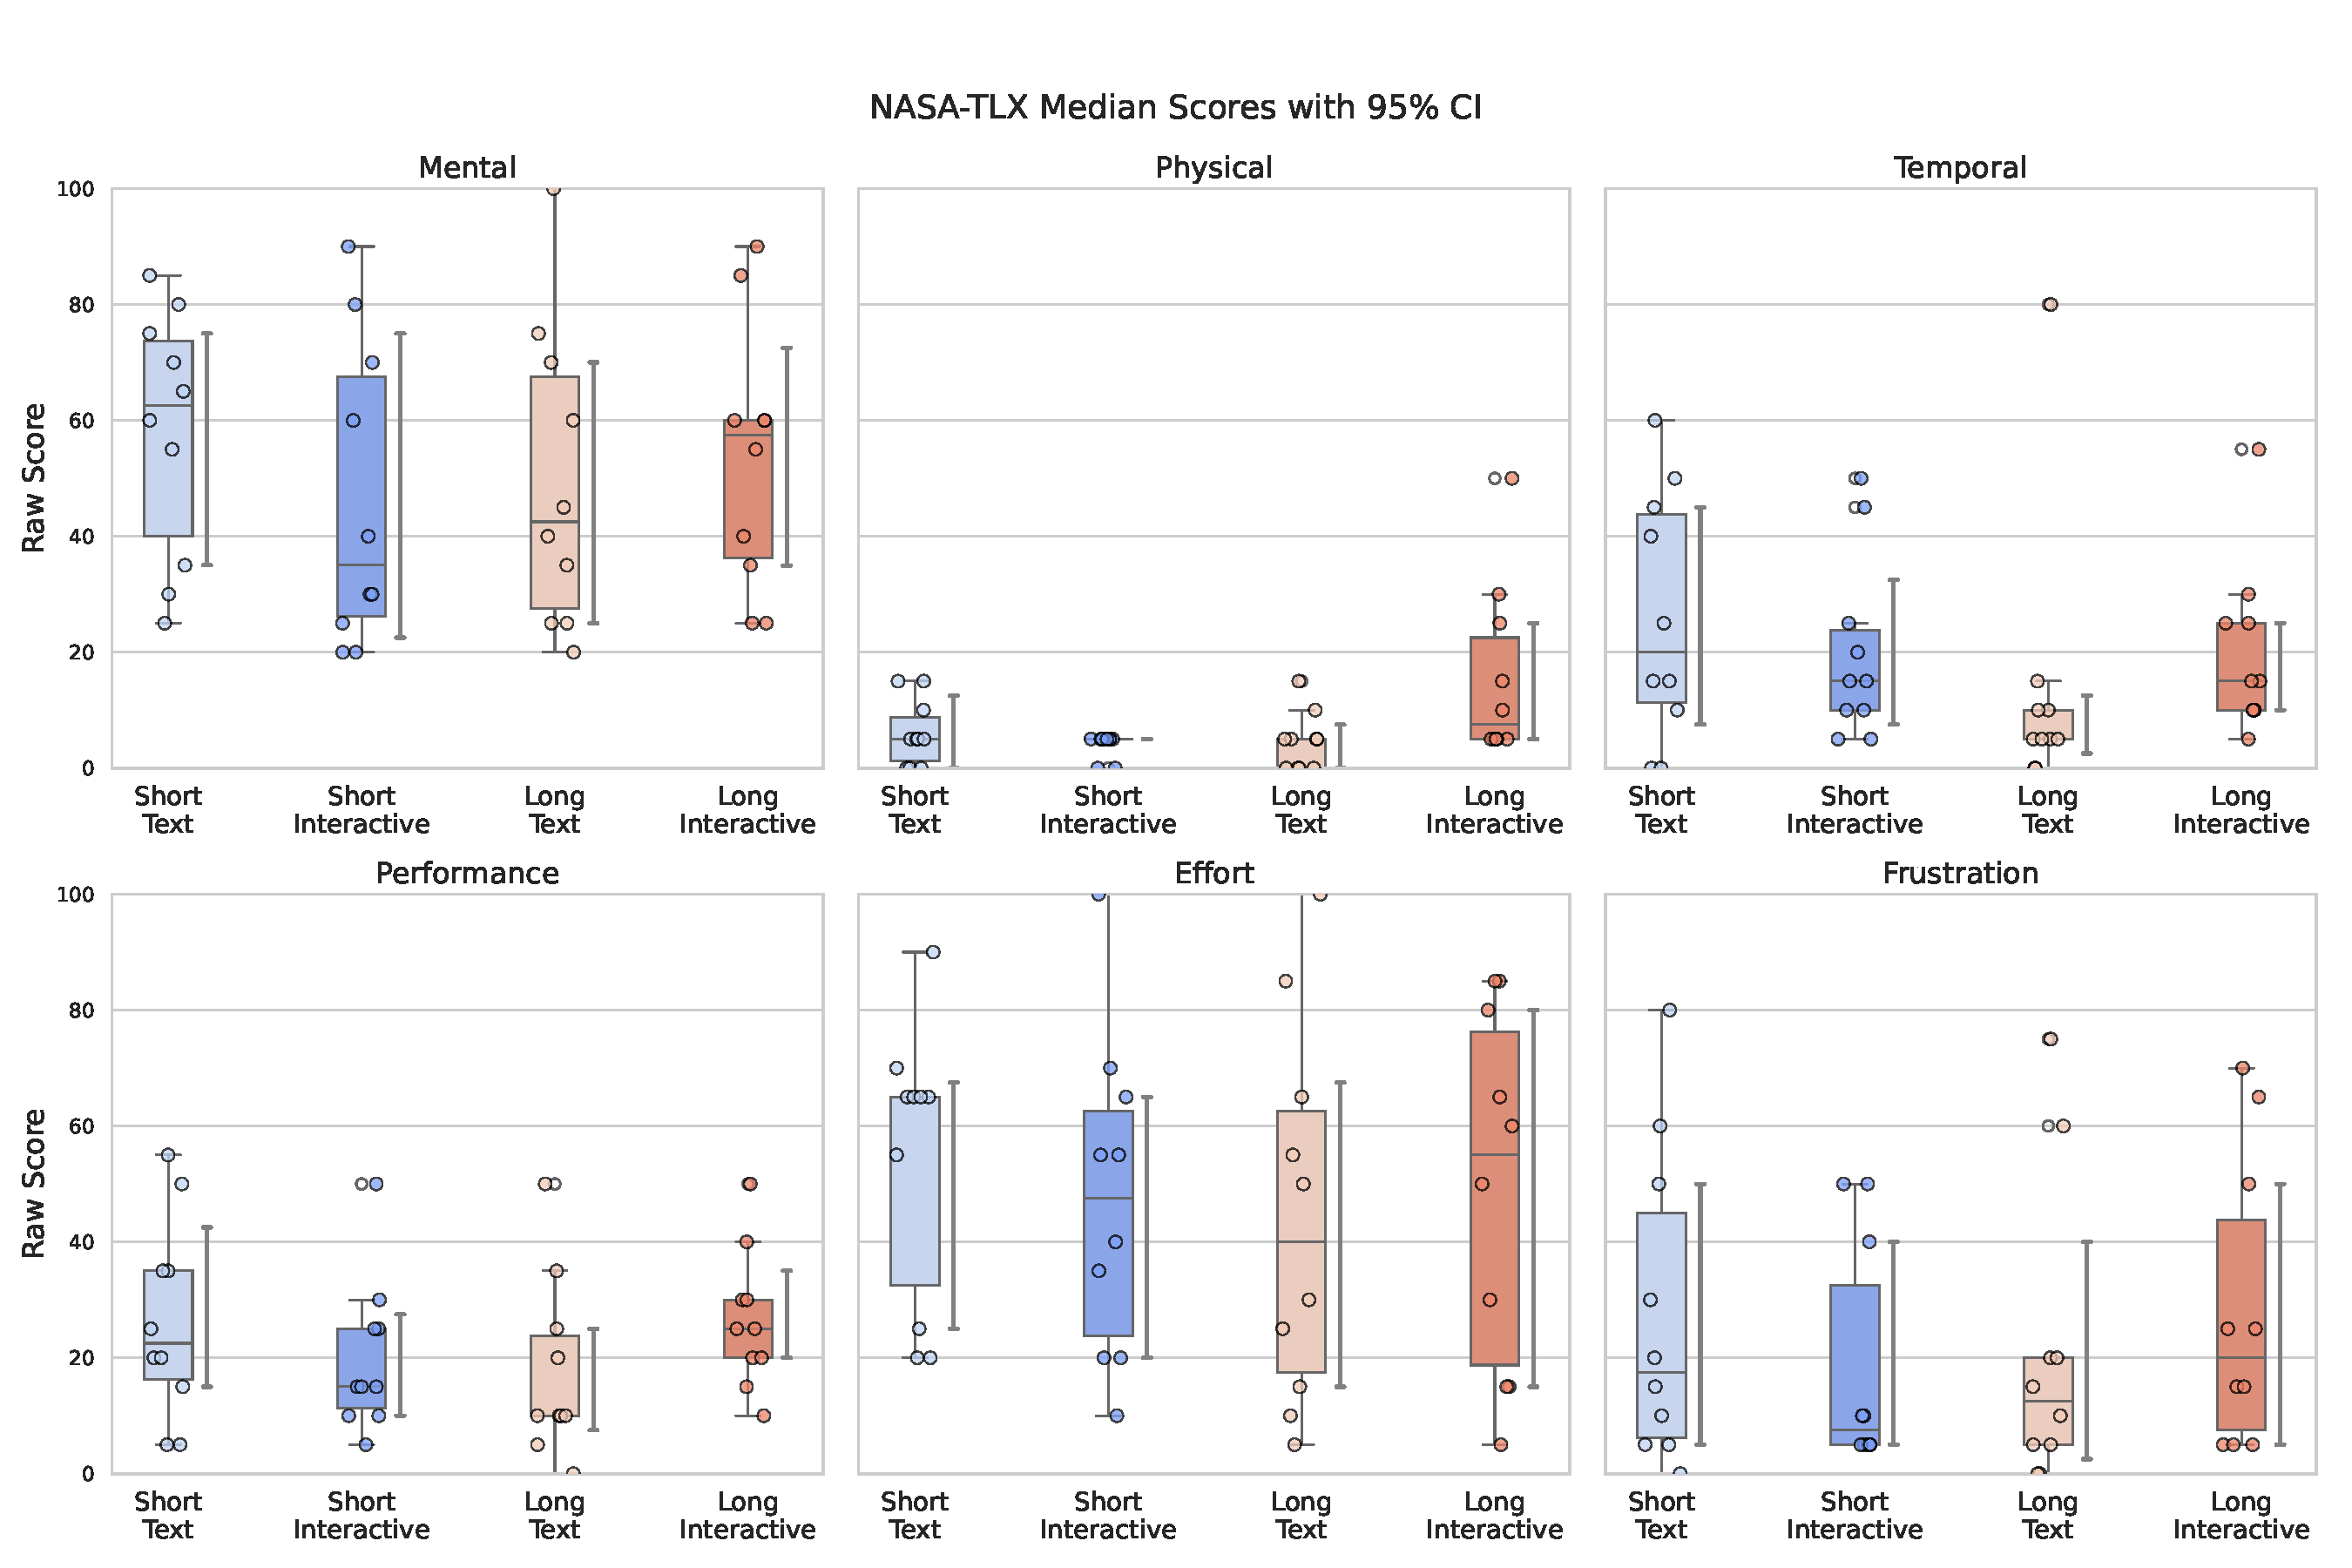
\includegraphics[width=\textwidth]{content/image/cog/nasatlx_final_value_with_CI.pdf}
%     \caption{NASA-TLX Results}
%     \label{fig:nasatlx-with-ci}
% \end{figure}





% Removed text yeard
%% Mental Demand

%\subsubsection{Mental Demand Source: Other Sources}
%We identified four additional sources causing participants' mental demands: \textit{experiment setup}, \textit{number of options}, \textit{QS mechanism}, and \textit{external factors}. 

%$24$ participants mentioned the experiment setup mainly related to understanding and recalling their experience with the options. $6$ participants, all from the long QS, found the number of options added mental demand. $4$ participants cited working with getting familiar with the QS mechanism as a source of mental demand. These are sources related to the study design. $12$ participants mentioned external factors, such as considering the consequences of their results or the challenges decision-makers face. $4$ participants reported an increase and another four a reduction in mental demand due to the interface design. $8$ participants expressed mental demand from justifying their choices and reflecting on their responses, questioning whether their votes truly reflected their preferences or if the amount of credit spent was justified.
% 
%In the first quote, participants felt mental demand focusing on three options, trying to recall specific characteristics to differentiate them. In the second quote, participants considered the societal impact of options, aiming to maximize their effect. This difference highlighted our belief that the organization phase prompted participants to consider a broader range of factors in their decisions. Across both interfaces, participants in the long survey tended towards operational mental demands related to budget management. 

% In addition, we also find that long text interface participants focused on more operational behaviors such as:

% \begin{displayquote}
% So I wanted to be fair.~\bracketellipsis I actually took my calculator out and said~\bracketellipsis  how much would it be if I equally distributed it and then how do I do that? Do I wanna do it all equally or not?

% \noindent \hfill -- S020, long text interface
% \end{displayquote}

% compared to more procedures involving more strategic planning such as:

% \begin{displayquote}
% I wanted to make sure I wanted to give some credit to everything~\bracketellipsis I'm trying to make sure that I had without doing a lot of~\ldots I guess redos is trying to kind of get it right the first time on how I weight things.

% \noindent \hfill -- S032, long two-phase interface
% \end{displayquote}



% IN_T4: Wanting more information on the options (N=6/40)
% 5. While the numbers seem small, non of this request came from v3. This could explain that participants are already overloaded from the existing the task.